\subsection{Camadas da Arquitetura Limpa}

     \begin{figure}[H] % O [H] exige o uso do pacote float (veja abaixo)
        \centering
        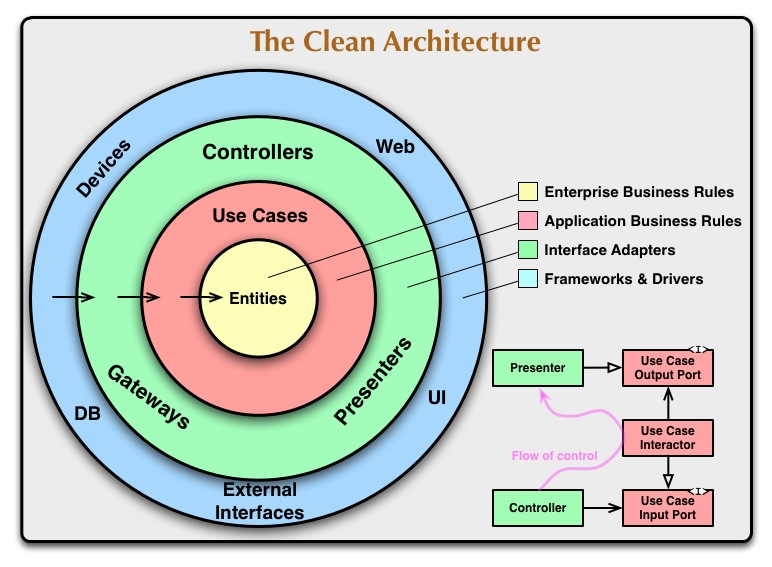
\includegraphics[width=0.8\textwidth]{figuras/clean_arch_1.jpg}
        \caption{A arquitetura limpa}
        \label{fig:figura_clean_arch_1}
        \newcommand{\minhafonteum}{Fonte: \cite{livro:martin:cleanarch}}
        \minhafonteum
    \end{figure}

    \par Para representar os princípios de separação de interesse e independência de detalhes, \cite{livro:martin:cleanarch} propõe um modelo visual para a Arquitetura Limpa, que pode ser visto na Figura \ref{fig:figura_clean_arch_1}, esse modelo define uma série de camadas concêntricas. Ele representa os níveis de abstração do software, indo desde as regras de negócio mais puras e de alto nível no centro, até os mecanismo e tecnologias na borda. A regra da dependência abordada anteriormente, dita a interação entre essas camadas, a seguir é detalhada cada uma dessas camadas:

    \begin{itemize}
        \item Entidades: As entidades são os componentes da arquitetura limpa responsáveis por encapsular as regras de negócio do software, sendo objetos ou coleções de dados e funções de tecnologias externas \cite{livro:martin:cleanarch, artigo:ferreira:2022, artigo:dantas:2021}. Elas fazem parte da camada central, que sofrera menos mudanças ao longo do tempo, e são a representação do domínio do sistemas. Além disso  as entidades garantem estabilidade, pois elas são desenvolvidas para não serem alteradas quando houver mudanças em interfaces ou bancos de dados \cite{artigo:dantas:2021, livro:martin:cleanarch};

        \item Casos de Uso: Os casos de uso são usados para realizar a implementação das regras de negócio específicas do software, orquestrando o fluxo de dados entre as entidades e outras camadas. Eles tem a característica de serem independentes de detalhes externos, com foco na intenção do negócio e também permitem que o desenvolvimento do software seja incremental e que os testes possam ser feitos de maneira isolada. \cite{artigo:ferreira:2022, livro:martin:cleanarch};

        \item Adaptadores de Interface: Os adaptadores de interface são responsáveis por converter dados de formatos internos (usado por casos de uso e entidades) e externos (como bancos de dados e APIs), eles servem para isolar os detalhes técnicos da lógica do negócio da aplicação, também são úteis para facilitar a substituição de tecnologias externas sem afetar as camadas mais internas do software \cite{livro:martin:cleanarch}. 

        \item Frameworks e Drivers: Os frameworks e drives representam as ferramentas e tecnologias externas, como bancos de dados, frameworks e dispositivos que fazem entrada ou saída de dados, considerado detalhes de implementação que podem mudar ao longo do tempo de desenvolvimento dos projetos \cite{livro:martin:cleanarch}.
    \end{itemize}